\documentclass[12pt,fleqn]{article}

\usepackage[utf8]{inputenc}
\usepackage[T2A]{fontenc}
\usepackage[english,russian]{babel}
\usepackage{graphicx}
\usepackage{indentfirst}
\usepackage{syntax}
\usepackage{amsmath}
\usepackage{titlesec}

\newcommand{\sectionbreak}{\clearpage}
\setcounter{secnumdepth}{0}

\begin{document}

\begin{titlepage}

\begin{center}
{\large
Санкт-Петербургский государственный университет информационных технологий, механики и оптики

Факультет информационных технологий и программирования

Кафедра «Компьютерные технологии»\\[3cm]

И.А.Иванов\\[2cm]}

{\large \bfseries
Отчет по курсовой работе\\[0.5cm]

«Генерация LTL-формул по конечному автомату с помощью генетического программирования»
}
\vfill

Санкт-Петербург

2015
\end{center}

\end{titlepage}

\tableofcontents

\section{Введение}

Темпоральная логика (\emph{Temporal Logic}) --- это логика, учитывающая причинно-следственные связи в условиях времени.
Используется для описания последовательностей явлений и их взаимосвязи по временной шкале.
Темпоральные логики часто применяются для выражения требований формальной верификации.
Например, свойства ``Если поступил запрос, то на него обязательно придет ответ''\ или
``Функция вызывается не более одного раза за вычисление''\ удобно формулировать с помощью темпоральных логик.
В линейной темпоральной логике (\emph{Linear Temporal Logic, LTL}) наряду с логическими операторами мы можем 
использовать следующие модальные операторы: утверждение истинно в следующем состоянии,
утверждение истинно всегда, утверждение когда-нибудь станет истинным,
одно утверждение будет истинным до тех пор, пока другое утверждение не станет истинным,
одно утверждение не станет ложным до тех пор (включительно), пока другое не станет истинным.

Задача нахождения спецификации (\emph{Specification mining}) --- задача построения формальной спецификации или модели
(обычно автоматной) для некоторой программы. В данной работе рассматривается способ построения спецификации
для управляющего конечного автомата в виде формул линейной темпоральной логики.
Управляющий конечный автомат характеризуется множеством состояний, входных событий, выходных воздействий,
а так же списком переходов, каждый из которых описывается начальным состоянием, конечным состоянием,
входным событием, булевой формулой от входных переменных и множеством выходных воздействий.
Базовыми утверждениями, которые мы будем использовать являются следующие: произошло входное событие
\emph{e}, произошло выходное воздействие \emph{z}. Таким образом, мы будем искать формулы, удовлетворяющие автомату,
обладающие также некоторыми дополнительными свойствами. Во-первых, мы хотим, чтобы сгенерированные
формулы давали нам как можно больше информации о входном автомате (в идеале полностью его описывали).
Во-вторых, генерируемые формулы предназначены для использования людьми, а значит не должны быть слишком громоздкими.
Позже эти требования будут формализованы.

В работе предлагается решение этой задачи с помощью генетического программирования --- класса алгоритмов,
которые решают задачи оптимизации путем подбора параметров с использованием механизмов, аналогичных естественному
отбору в природе, --- мутации, отбора и скрещивания. Чаще всего особи в генетическом программировании представляют
в виде дерева. Оператор скрещивания реализуется обменом между двумя деревьями какими-либо узлами вместе с их
потомками. Оператор мутации может быть реализован изменением информации в узле, добавлением или удалением узла
или целого поддерева. Пусть, например, особи являются деревьями разбора формул пропозициональной логики.
Тогда оператор скрещивания для формул
$$
(a \vee b) \rightarrow (a \wedge b \vee c)
$$
$$
(b \wedge c) \vee (b \rightarrow (\lnot c \wedge a))
$$
мог бы выдать следующие результаты:
$$
(b \wedge c) \rightarrow (a\wedge b \vee c)
$$
$$
(b \wedge c) \vee (b \rightarrow (a \wedge b))
$$
$$
(b \rightarrow (\lnot c \wedge a)) \rightarrow (a \wedge b \vee c)
$$
А результатом применения оператора мутации к формуле
$$
(a \rightarrow b) \rightarrow (\lnot c \wedge (b \rightarrow a))
$$
могут быть следующие формулы:
$$
(a \wedge b) \rightarrow (\lnot c \wedge (b \rightarrow a))
$$
$$
(c \vee a) \rightarrow (\lnot c \wedge (b \rightarrow a))
$$
$$
(a \rightarrow b) \rightarrow (\lnot (a \rightarrow \lnot b) \wedge (b \rightarrow a))
$$
$$
(a \rightarrow b) \rightarrow c
$$

\section{1. Постановка задачи}

В работе управляющим конечным автоматом будем называть семерку $\langle X,\; E,\; Y,\; Z,\; y_0,\; \phi,\; \delta \rangle$,
где $X$ --- множество входных булевых переменных; $E$ --- множество событий; $Y$ --- множество состояний;
$y_0 \in Y$ --- начальное состояние; $Z$ --- множество выходных воздействий;
$\phi : Y \times E \times 2^x \rightarrow Y$ --- функция переходов, а
$\delta : Y \times E \times 2^X \rightarrow Z^*$ --- функция выходов.

\begin{figure}[!hb]
  \centering
    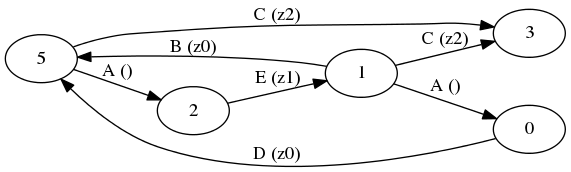
\includegraphics[scale=0.5]{lift.png}
  \caption{Пример управляющего автомата.}
\end{figure}

Язык LTL состоит пропозициональных переменных, логических операторов $\wedge,\; \vee,\; \lnot,\; \rightarrow$\ и набора
темпоральных операторов, таких как, например, $G$\ (Глобально в будущем), $X$\ (В следующий момент времени) и
$F$\ (когда-либо в будущем). Ниже приведена формула, утверждающая, что всегда в будущем из того, что верно $B$, следует,
что когда-либо в будущем будет верно $A$, и в следующий момент времени верно $C$.

$$
G(B \rightarrow F(A)) \wedge X(C)
$$

Пусть задан входной автомат $a$. Требуется найти удовлетворяющие ему формулы, оптимальные в смысле ранее указанных
двух свойств. Формализуем их.

Пусть $A_f$ --- множество всех возможных автоматов, удовлетворяющих некоторой формуле $f$. Будем считать,
что чем меньше мощность $A_f$, тем больше информации о входном автомате $a$ несет формула.

Пусть есть множество операторов $O$ и множество базовых утверждений $S$.
Тогда каждому опреатору $o \in O$ и утверждению $s \in S$ сопоставим его вес $w_o$ и $w_s$ соответственно.
Введем понятие веса формулы таким образом: $\text{weight}(s) = w_s$, $\text{weight}(o(arg_1\; \ldots \; arg_n)) = w_o + \sum_{i=1}^{n}\text{weight}(arg_i)$.
Будем искать формулы минимального веса, формализовав таким образом требование простоты формулы.

\section{2. Предлагаемый алгоритм}

Для решения задачи будем использовать генетическое программирование\cite{kz1}. Будем преставлять формулу в виде дерева разбора.
Для генерации, скрещивания и мутации формул будем использовать стандартные алгоритмы генетического программирования,
реализованные в библиотеке эволюционных алгоритмов ECJ (http://cs.gmu.edu/~eclab/projects/ecj) и описанные в \cite{kz1,kz2}.
Tак как в качестве целевых были выделены сразу несколько критериев, то будем использовать многокритериальную оптимизацию.

Многокритериальная оптимизация --- это процесс одновременной оптимизации двух или более конфликтующих целевых функций
в заданной области определения. В качестве критерия оптимальности будем использовать оптимальность по Парето:
Говорят, что одно решение доминирует над другим, если оно по всем критериям не хуже другого и как минимум по одному
строго лучше. Множеством оптимальных решений называются решения, над которыми никто не доминирует. Таким образом
в качестве результата работы алгоритма будет получен фронт решений, являющихся оптимальными. В качестве конкретных
реализаций многокритериальной оптимизации были испробованны алгоритмы NSGA2\cite{nsga2} и SPEA2\cite{spea2}.
При одинаковых результатах SPEA2 работал существенно быстрее и был выбран для использования. Алгоритм SPEA2
наряду с популяцией использует архив. Начав с пустым архивом $A_0$ и сгенрированной популяцией $P_0$, алгоритм до
тех пор, пока не выполнено одно из завершающих условий, выполняет следующие шаги: Назначить каждой особи $i$ из $P_t$ и $A_t$
значение функции приспособленности
$$
F(i) = \frac{1}{d_k(i) + 2} + \sum_{j\in P_t + A_t, j > i}|\{k|k \in P_t + A_t \wedge k > j\}|
$$
Где $d_k$ --- расстояние до k-ой ближайшей особи (обычно берут $k = \sqrt{|P| + |A|}$), > --- отношение доминирования по Парето. Скопировать оптимальные
особи из $P_t$ и $A_t$ в $P_{t+1}$ (при необходимости архив обрезается или дополняется неоптимальными решениями).
С помощью бинарного турнира выбрать особи из $A_{t+1}$ для скрещивания с целью получения новой популяции. 

В качестве критериев оптимизации будем использовать: верность формулы для входного автомата, минимальность веса
формулы и минимальность числа автоматов, которым удовлетворяет формула. Очевидно, однако, что вычисление последнего
критерия не представляется возможным даже для небольшого числа состояний в автомате. Поэтому в дальнейшем будут
рассмотренны несколько критериев и их комбинаций, эффективно приближающих требуемое. Позже будет приведен
анализ качества их работы.

Будем генерировать формулы вида $G(\ldots)$ ввиду того, что нас интересуют свойства автомата, которые выполняются
в любой момент времени. Система типов ECJ позволяет сопоставить каждому узлу дерева особи его тип. Тип узла
определяет количество и типы его поддеревьев. ECJ будет генерировать только корректно типизирующиеся особи.
Таким образом мы можем накладывать на них определенные ограничения. В частности мы запретим генерацию следующих
комбинаций: $\lnot(\lnot(\ldots))$, $F(F(\ldots))$, $F(X(\ldots))$, $X(F(\ldots))$, $G(X(\ldots))$, так как
они имеют более простые аналоги, ничем или слабо отличающиеся с точки зрения смысла.

\subsection{Критерий 1. Входной автомат должен удовлетворять формуле.}

Будем определять удовлетворяет ли формула $f$ автомату $a$ с помощью верификатора автоматных программ, разработанного в \cite{eg}.
При этом такая проверка будет возвращать число $r(a, f) = \frac{\text{verifiedTransitions}(a, f)}{\text{totalTransitions}(a)}$ --- отношение числа
переходов, которым формула удовлетворяет, к общему числу переходов. Таким образом $r(a, f)$ лежит в промежутке $[0, 1]$\ и равно
еденице, когда формула удовлетворяет автомату.

\subsection{Критерий 2. Минимальность веса формулы.}

Ранее для каждой формулы $f$ был введен ее вес $\text{weight}(f)$. Используем в качестве критерия число $c = \frac{1}{\text{weight}(f)}$.
В качестве весов операторов и утверждений выберем числа большие или равные еденице.
В таком случае $c \in [0, 1]$ и максимально при минимальном весе формулы.

\subsection{Критерий 3. Число случайных автоматов, удовлетворяющих формуле.}

Сгенерируем некоторое число $N$ случайных автоматов с теми же множествами состояний, входных и выходных событий, что и
у исходного. Для каждого из полученных автоматов измерим с помощью верификатора насколько формула ему уовлетворяет.
Получим $N$ чисел $r_i$ из промежутка $[0, 1]$. В качестве результата возьмем велечину $c = \frac{1}{1 + \sum_{i = 1}^{N}r_i^2}$.

\subsection{Критерий 4. Число мутантов исходного автомата, удовлетворяющих формуле.}

Возьмем исходный автомат и сгенерируем для него некоторое количество мутантов --- исходных автоматов с небольшими
случайными изменениями функций переходов $\phi$ и выходов $\delta$. Будем использовать следующие операторы мутации:

1. \textbf{Изменение состояния в которое ведет переход.} Для случайно выбранного перехода в автомате состояние $y$,
в которое он ведет, заменяется на другое состояние, случайно выбранное из $Y \textbackslash \{y\}$. 

2. \textbf{Добавление или удаление переходов.} Для каждого состояния с определенной вероятностью изменим набор переходов.
Случайным образом решается добавить или удалтить переход. В случае добавления перехода добавим новый переход из
текущего состояния в некоторое случайно выбранное состояние. В случае удаления из текущего состояния удаляется
случайно выбранный переход.

В качестве результата используем величину, аналогичную результату для случайных автоматов.

\subsection{Критерий 5. Удовлетворение формулы автомату, построенному по сценариям.}

Сценарий --- некоторый случайный путь фиксированной длины в автомате. Построим для входного автомата некоторое
число сценариев. На основе этих сценариев построим новый автомат $a^*$ при помощи способа, описанного в \cite{eg}.
Заметим, что полученный автомат может удовлетворять не всем формулам, верным для исходного автомата, так как
длина любого сценария конечна. В качестве результата используем велечину $1 - r(a^*, f)$.

\subsection{Критерий 6. Число мутантов автомата, построенного по сценариям, удовлетворяющих формуле.}

Критерий аналогичен критерию номер четыре с тем лишь отличием, что мутанты строятся на основе автомата, построенного по
сценариям, а не исходного.

\section{3. Результаты}

\subsection{Проведенные испытания}

Для тестирования алгоритма использовался автомат, управляющий дверьми лифта, описанный в \cite[Sec 2.3.1]{eg}.

\begin{figure}[!hb]
  \centering
    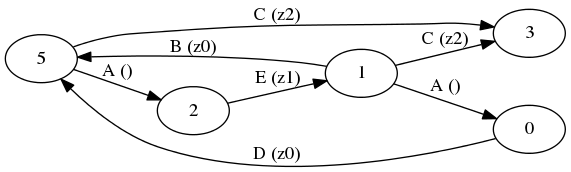
\includegraphics[scale=0.5]{lift.png}
  \caption{Автомат, управляющий дверьми лифта.}
\end{figure}

Состояние под номером ноль --- начальное. Автомат принимает следующие события:

$\bullet$ $A$ --- двери лифта полностью открылись или закрылись;

$\bullet$ $B$ --- закрытию дверей мешает препятствие;

$\bullet$ $C$ --- поломка дверей лифта;

$\bullet$ $D$ --- нажата кнопка ``Открыть двери'';

$\bullet$ $E$ --- нажата кнопка ``Закрыть двери''.

Автомат имеет три выходных воздействия:

$\bullet$ $z0$ --- приступить к открытию дверей;

$\bullet$ $z1$ --- приступить к закрытию дверей;

$\bullet$ $z2$ --- сообщить в аварийную службу о поломке лифта.

Автомат был построен на основе следующей спецификации:
\begin{multline*}
G(\text{wasEvent}(D) \rightarrow \text{wasAction}(z0))\\
G(\text{wasEvent}(E) \leftrightarrow \text{wasAction}(z1))\\
G(\text{wasEvent}(C) \leftrightarrow \text{wasAction}(z2))\\
G(\text{wasEvent}(B) \rightarrow \text{wasAction}(z0))\\
G(\text{wasEvent}(A) \rightarrow X(\text{wasEvent}(D) \vee \text{wasEvent}(E)))\\
G(\text{wasEvent}(D) \rightarrow X(\text{wasEvent}(A) \vee \text{wasEvent}(C)))\\
G(\text{wasAction}(z0) \rightarrow X(\text{wasEvent}(A) \vee \text{wasEvent}(C)))\\
G(\text{wasEvent}(E) \rightarrow X(\text{wasEvent}(A) \vee \text{wasEvent}(B) \vee \text{wasEvent}(C)))\\
G(\text{wasAction}(z0) \rightarrow X(U(\lnot \text{wasAction}(z0), \text{wasAction}(z1) \vee \text{wasEvent}(C))))\\
G(\text{wasAction}(z1) \rightarrow X(U(\lnot \text{wasAction}(z1), \text{wasAction}(z0) \vee \text{wasEvent}(C))))\\
\lnot F(\text{wasEvent}(C) \wedge X(F(\text{wasEvent}(D) \vee \text{wasEvent}(E) \vee \\ \vee \text{wasEvent}(A) \vee \text{wasEvent}(B) \vee \text{wasEvent}(C))))
\end{multline*}

Проведено несколько запусков различных конфигураций алгоритма. Во всех конфигурациях использовались первые два критерия.
Для оставшихся четырех критериев были испытанны все комбинации. Всего таким образом было получено шестнадцать конфигураций.
Число поколений в каждом испытании --- 50, размер популяции --- 500, размер архива --- 100.

\begin{table}
\centering
\begin{tabular}{ l | l | l | l | l | l | l }
конфигурация \textbackslash \ критерий & 1 & 2 & 3 & 4 & 5 & 6 \\
1  & + & + & - & - & - & - \\
2  & + & + & - & - & - & + \\
3  & + & + & - & - & + & - \\
4  & + & + & - & - & + & + \\
5  & + & + & - & + & - & - \\
6  & + & + & - & + & - & + \\
7  & + & + & - & + & + & - \\
8  & + & + & - & + & + & + \\
9  & + & + & + & - & - & - \\
10 & + & + & + & - & - & + \\
11 & + & + & + & - & + & - \\
12 & + & + & + & - & + & + \\
13 & + & + & + & + & - & - \\
14 & + & + & + & + & - & + \\
15 & + & + & + & + & + & - \\
16 & + & + & + & + & + & + \\
\end{tabular}
\caption{Конфигурации.}
\end{table}

Для оценки результатов будем, во-первых, анализировать полученные формулы вручную. Формулы, сообщающие некоторые тривиальные
факты, например: ``В любой момент времени либо что-то мешает закрытию дверей либо нет'', нас не интересуют.
Так же не подходят чрезмерно сложные и громоздкие формулы. Примером хороших формул может служить приведеная ранее спецификация.

Во-вторых, наряду с анализом полученных формул вручную будем использовать следующую велечину:
Построим на основе выведенных формул и сценариев автомат. Возьмем набор формул, написанных человеком для исходного автомата, и
проверим сколько из них удовлетворяют построенному автомату. Чем больше эта величина, тем больше информации об исходном
автомате нам дают выведенные формулы.

\subsection{Результаты испытаний}

Было проведено десять запусков каждой из шестнадцати конфигураций. Суммарное время работы составило чуть менее семнадцати часов.
Спецификация, содержащая семнадцать формул была взята из \cite{eg}.
Таким образом то, насколько много информации дают формулы, полученные с помощью некоторой конфигурации, о входном автомате,
характеризуется числом от 0 до 170.

Максимальный результат --- 170 набрала реализация номер шестнадцать. Второе место с результатом 169 разделили две реализации:
номер десять и номер четырнадцать. Третье место (164) так же заняли две реализации: номера семь и двенадцать.
Далее приведены примеры сгенерированных формул: 

\begin{multline*}
G(F(\text{wasAction}(z1)) \rightarrow \lnot \text{wasAction}(z2))\\
G(X(\text{wasAction}(z1)) \rightarrow \text{wasEvent}(A))\\
G(\text{wasAction}(z0) \rightarrow F(\text{wasAction}(z1) \vee X(\text{wasAction}(z2))))\\
G(X(\text{wasEvent}(A)) \rightarrow (\text{wasAction}(z1) \vee \text{wasAction}(z0)))\\
\end{multline*}

\section{4. Заключение}

Разработан метод генерации LTL-формул по управляющему конечному автомату и написана программа на языке программирования Java
(https://github.com/V1489Cygni/ltlgen), являющаяся модулем для библиотеки ECJ и реализующая этот метод.
Были протестированны различные конфигурации алгоритма и выбранны лучшие из них. При тестированнии алгоритм показал
достаточно стабильные результаты, было получено достаточное количество формул, удовлетворяющих поставленной цели.

\begin{thebibliography}{5}

\bibitem{kz1}John R. Koza. Genetic Programming: On the Programming of Computers by Means of Natural Selection. MIT press, 1992.

\bibitem{kz2}John R. Koza. Genetic Programming II: Automatic Discovery of Reusable Programs. MIT press, 1994.

\bibitem{nsga2}Kalyanmoy Deb, Amrit Pratap, Sameer Agarwal, T. Meyarivan. A Fast and Elitist Multiobjective Genetic Algorithm: NSGA-II.

\bibitem{spea2}Eckart Zitzler, Marco Laumanns, Lothar Thiele. SPEA2: Improving the Strength Pareto Evolutionary Algorithm. //
Computer Engineering and Networks Laboratory (TIK)
Department of Electrical Engineering
Swiss Federal Institute of Technology (ETH) Zurich
ETH Zentrum, Gloriastrasse 35, CH-8092 Zurich, Switzerland.

\bibitem{eg}Егоров Кирилл Викторович. Генерация управляющих автоматов на основе генетического программирования и верификации: 
Диссертация на соискание ученой степени кандидата технических наук. 2013.   

\end{thebibliography}

\end{document}
